\chapter{配体场理论与颜色}\label{ch:b2:ligand-field}

红宝石是红色的，祖母绿是绿色的，但两者的颜色都来自同一种离子，
\ce{Cr^3+}，其中少量取代刚玉 \ce{Al2O3} 中的铝，或
取代绿柱石中的铝。硫酸铜晶体呈深蓝色，而加热后残留的
粉末为白色。两种情况下，颜色都源于电子在
d 轨道之间跃迁，这些轨道的能量已被周围原子拉开——
拉开的幅度取决于包围离子的原子种类及其排布方式。本
章先用点电荷、再用分子
轨道计算这种分裂；并解释颜色、磁性，以及
上一章的 18 电子规则。

\begin{recall}
\Cref{ch:b2:coordination-complexes}：$d^n$ 组态、几何构型与电子
计数。\Cref{ch:b2:atomic-orbitals}：五个 d 轨道的形状。
\Cref{ch:b2:fragment-orbitals}：片段轨道。本科一年级分册：吸光度、
互补色、未成对电子、洪特规则。
\end{recall}

\begin{omfigure}
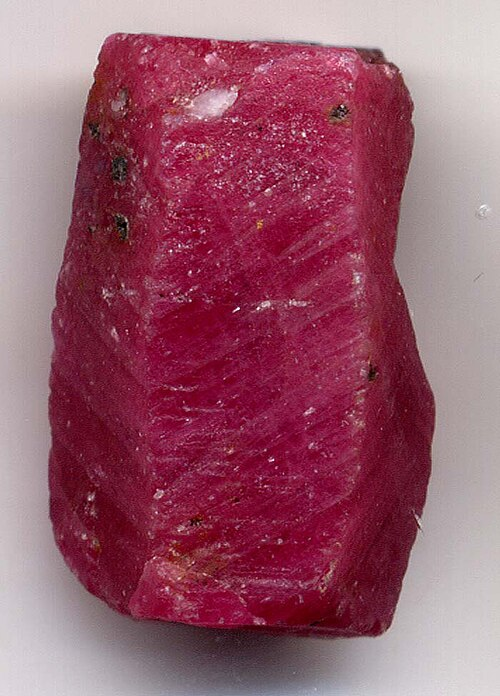
\includegraphics[height=3.6cm]{images/book3/ruby.jpg}\hspace{0.6cm}%
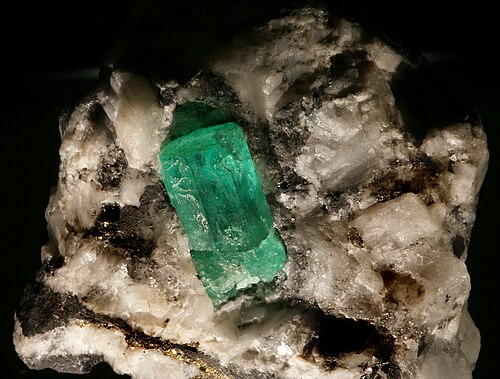
\includegraphics[height=3.6cm]{images/book3/emerald.jpg}\hspace{0.6cm}%
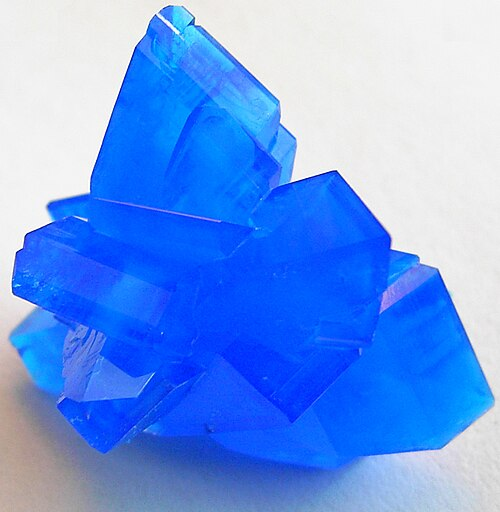
\includegraphics[height=3.6cm]{images/book3/copper-sulfate.jpg}

{\small 红宝石晶体（公有领域）；岩石中的祖母绿（Didier Descouens，
CC BY-SA 3.0）；五水硫酸铜(II)晶体（Stephanb，CC BY-SA
3.0）。维基共享资源。铬(III)使前两者着色，而
铜(II)的水合配合物使第三者着色。}
\end{omfigure}

\section{晶体场模型}

\begin{definition}[晶体场]\label{def:b2:ligand-field:crystal-field}
\emph{晶体场模型}\index{晶体场模型}把
配合物的配体视为环绕金属
离子的负点电荷（或偶极子的负端），并计算它们如何改变其 d 轨道的能量。在八面体
场中，d 轨道分裂为两组，两组之间的\emph{晶体场
分裂}\index{晶体场分裂} $\Delta_o$。
\end{definition}

将六个配体置于坐标轴上。$\mathrm d_{z^2}$ 与 $\mathrm d_{x^2-y^2}$
轨道的瓣直指配体，其中电子受到的排斥更强，
能量随之升高。$\mathrm d_{xy}$、$\mathrm d_{xz}$、$\mathrm d_{yz}$ 轨道的瓣
位于配体之间，升高较少。第一对称为 $e_g$，第二组三个轨道
称为 $t_{2g}$（名称来自群论，见本科三年级分册）。

\begin{omfigure}
\begin{tikzpicture}[font=\small]
  \begin{scope}
    \pic at (0,0) {omdx2y2};
    \foreach \p in {(1.25,0),(-1.25,0),(0,1.25),(0,-1.25)} \node[circle, fill=black!70, inner sep=2.2pt] at \p {};
    \node at (0,-1.75) {$\mathrm d_{x^2-y^2}$：瓣指向配体};
  \end{scope}
  \begin{scope}[xshift=5.5cm]
    \pic at (0,0) {omdxy};
    \foreach \p in {(1.25,0),(-1.25,0),(0,1.25),(0,-1.25)} \node[circle, fill=black!70, inner sep=2.2pt] at \p {};
    \node at (0,-1.75) {$\mathrm d_{xy}$：瓣位于它们之间};
  \end{scope}
\end{tikzpicture}

{\small 八面体 $xy$ 平面内四个配体之间的两个 d 轨道
（黑点）。$\mathrm d_{x^2-y^2}$ 的瓣指向配体，而
$\mathrm d_{xy}$ 的瓣位于它们之间。}
\end{omfigure}

\begin{theorem}[重心]\label{thm:b2:ligand-field:barycentre}
在八面体场中，以 d 轨道的平均能量为参照，
$e_g$ 组位于 $+0.6\Delta_o$，$t_{2g}$ 组位于 $-0.4\Delta_o$。
\end{theorem}

\begin{proof}
场使五个 d 轨道能量的平均值升高，但分裂
并不改变这一平均值（重心规则，在本阶段不加证明地承认：一整套轨道的能量位移之和
只由总电荷决定，与排布无关）。令 $e_g$ 位于 $x$，
$t_{2g}$ 位于 $x - \Delta_o$，于是由条件 $2x + 3(x - \Delta_o) = 0$ 得 $x = 0.6\Delta_o$。
\end{proof}

\section{高自旋与低自旋}

\begin{definition}[自旋态]\label{def:b2:ligand-field:spin}
\emph{成对能}\index{成对能} $P$ 指将第二个
电子放入已占据的轨道（而非同能量的空轨道）所需的能量。若
配合物为\emph{高自旋}\index{高自旋}，即其电子先占据 $e_g$ 轨道，
而后才在 $t_{2g}$ 中成对；\emph{低自旋}\index{低自旋}则是
电子先在 $t_{2g}$ 中成对。
\end{definition}

\begin{proposition}[自旋态的选择]\label{prop:b2:ligand-field:spin-state}
对于八面体场中的 $d^4$ 至 $d^7$ 离子，$\Delta_o > P$ 时配合物为低自旋，
$\Delta_o < P$ 时为高自旋。对于 $d^1$--$d^3$ 与 $d^8$--$d^{10}$，只存在一种组态。
\end{proposition}

\begin{proof}
由 $d^3$（$t_{2g}^3$）出发，第四个电子要么进入 $e_g$（代价为 $\Delta_o$，
即高出 $t_{2g}$ 的部分），要么在 $t_{2g}$ 中成对（代价为 $P$）。代价较小者胜出，同样的比较
对每个电子直至 $d^7$ 均成立。对于 $d^1$--$d^3$，$t_{2g}$ 中有足够空间，无需成对；
对于 $d^8$--$d^{10}$，$t_{2g}$ 已满，必须占用 $e_g$。
\end{proof}

\begin{definition}[晶体场稳定化能]\label{def:b2:ligand-field:cfse}
称\emph{晶体场稳定化能}\index{晶体场稳定化能}
（CFSE）为组态 $t_{2g}^ae_g^b$ 的 $(-0.4a + 0.6b)\Delta_o$，即
d 电子相对于重心的能量（成对能另行计算）。
\end{definition}

\begin{proposition}[沿系列的晶体场稳定化能]\label{prop:b2:ligand-field:cfse}
高自旋时，CFSE 依次为 $0$、$-0.4$、$-0.8$、$-1.2$、$-0.6$、$0$、$-0.4$、$-0.8$、$-1.2$、
$-0.6$、$0$（以 $\Delta_o$ 为单位），对 $d^0$ 至 $d^{10}$ 而言，它在 $d^0$、$d^5$、$d^{10}$ 时为零。低
自旋时，它达到 $-2.4\Delta_o$，对应 $d^6$。
\end{proposition}

\begin{proof}
填入各组态并应用定义；所列数值与图中一致，
均经计算得出。
\end{proof}

\begin{omfigure}
\begin{tikzpicture}
\begin{axis}[width=0.55\linewidth, height=5cm, xmin=-0.5, xmax=10.5, ymin=-2.6, ymax=0.3,
  axis x line=bottom, axis y line=left, xlabel={$d^n$}, ylabel={晶体场稳定化能（$\Delta_o$）},
  xtick={0,1,2,3,4,5,6,7,8,9,10}, tick label style={font=\small}, label style={font=\small}]
\addplot[omThm, thick, mark=*, mark size=1.3pt] table[x=n, y=high] {figdata/out/bachelor-2-ligand-field-a.dat};
\addplot[omDef, thick, dashed, mark=square*, mark size=1.3pt] table[x=n, y=low] {figdata/out/bachelor-2-ligand-field-a.dat};
\node[font=\scriptsize, omThm, anchor=west] at (axis cs:5.4,0.0) {高自旋};
\node[font=\scriptsize, omDef, anchor=west] at (axis cs:6.6,-2.2) {低自旋};
\end{axis}
\end{tikzpicture}\hfill
\begin{tikzpicture}[font=\small]
  \pic (t) at (0,0) {omlevel={ud}{0.5}}; \pic at (0.6,0) {omlevel={u}{0.5}}; \pic at (1.2,0) {omlevel={u}{0.5}};
  \pic at (0.3,1.6) {omlevel={u}{0.5}}; \pic at (0.9,1.6) {omlevel={u}{0.5}};
  \node at (0.6,-0.8) {高自旋 $d^6$};
  \node[font=\scriptsize, anchor=east] at (-0.35,0) {$t_{2g}$}; \node[font=\scriptsize, anchor=east] at (-0.05,1.6) {$e_g$};
  \pic at (3,0) {omlevel={ud}{0.5}}; \pic at (3.6,0) {omlevel={ud}{0.5}}; \pic at (4.2,0) {omlevel={ud}{0.5}};
  \pic at (3.3,2.4) {omlevel={empty}{0.5}}; \pic at (3.9,2.4) {omlevel={empty}{0.5}};
  \node at (3.6,-0.8) {低自旋 $d^6$};
  \draw[<->, omProp] (4.7,0) -- (4.7,2.4) node[midway, right, font=\scriptsize] {$\Delta_o$};
  \draw[<->, omProp] (1.7,0) -- (1.7,1.6) node[midway, right, font=\scriptsize] {$\Delta_o$};
\end{tikzpicture}

{\small 左：沿 d 系列的晶体场稳定化能（经计算），
高自旋（实线）与低自旋（虚线）。右：一个 $d^6$
离子的两种组态：当 $\Delta_o < P$ 时有四个未成对电子（如 \ce{[Fe(H2O)6]^2+}），当 $\Delta_o >
P$ 时无未成对电子（如 \ce{[Fe(CN)6]^4-}）。}
\end{omfigure}

\begin{method}[自旋态、晶体场稳定化能与未成对电子]\label{met:b2:ligand-field:spin-state}
\begin{enumerate}
  \item 由氧化数求 $n$（$n = g - m$）。
  \item 对 $d^4$--$d^7$，比较 $\Delta_o$ 与 $P$（或将配体置于
        光谱化学序列中）：强场低自旋，弱场高自旋。
  \item 相应地填充 $t_{2g}$ 与 $e_g$；晶体场稳定化能 $= (-0.4a + 0.6b)\Delta_o$。
  \item 数出未成对电子；只要存在一个未成对电子，配合物即具有
        顺磁性。
\end{enumerate}
\end{method}

\section{其他几何构型}

\begin{proposition}[四面体场与平面正方形场]\label{prop:b2:ligand-field:tetrahedral}
在四面体场中能级次序颠倒：两个轨道（$e$）低于三个轨道（$t_2$），
同一金属与配体时，分裂能 $\Delta_t \approx \frac49\Delta_o$；四面体
配合物为高自旋。在平面正方形场中，$\mathrm d_{x^2-y^2}$ 轨道远高于其他轨道：
一个 $d^8$ 离子填满其余四个较低轨道，该轨道则保持空置。
\end{proposition}

\admitted

因子 $4/9$ 来源于点电荷的几何构型；由于仅有四个配体，
且无一配体位于坐标轴方向，分裂太小，不足以克服成对
能。将八面体中位于 $z$ 轴上的两个配体移去，使含 $z$ 分量的轨道降低，
而不抬高任何轨道：这解释了上一章中的平面正方形 $d^8$ 配合物，
其八个电子都能在空的
$\mathrm d_{x^2-y^2}$ 轨道之下找到位置。

\begin{omfigure}
\begin{tikzpicture}[font=\scriptsize]
  % octahedral
  \pic at (-0.3,0) {omlevel={empty}{0.45}}; \pic at (0.25,0) {omlevel={empty}{0.45}}; \pic at (0.8,0) {omlevel={empty}{0.45}};
  \pic at (0,1.8) {omlevel={empty}{0.45}}; \pic at (0.55,1.8) {omlevel={empty}{0.45}};
  \node[anchor=west] at (1.1,0) {$t_{2g}$}; \node[anchor=west] at (0.85,1.8) {$e_g$};
  \node[font=\small] at (0.25,-0.7) {八面体};
  % tetrahedral
  \begin{scope}[xshift=3.5cm]
    \pic at (0,0.6) {omlevel={empty}{0.45}}; \pic at (0.55,0.6) {omlevel={empty}{0.45}};
    \pic at (-0.3,1.4) {omlevel={empty}{0.45}}; \pic at (0.25,1.4) {omlevel={empty}{0.45}}; \pic at (0.8,1.4) {omlevel={empty}{0.45}};
    \node[anchor=west] at (0.85,0.6) {$e$}; \node[anchor=west] at (1.1,1.4) {$t_2$};
    \node[font=\small] at (0.25,-0.7) {四面体};
  \end{scope}
  % square planar
  \begin{scope}[xshift=7cm]
    \pic at (0,-0.2) {omlevel={empty}{0.45}}; \pic at (0.55,-0.2) {omlevel={empty}{0.45}};
    \pic at (0.25,0.3) {omlevel={empty}{0.45}};
    \pic at (0.25,0.9) {omlevel={empty}{0.45}};
    \pic at (0.25,2.6) {omlevel={empty}{0.45}};
    \node[anchor=west] at (0.85,-0.2) {$\mathrm d_{xz}, \mathrm d_{yz}$};
    \node[anchor=west] at (0.55,0.3) {$\mathrm d_{z^2}$};
    \node[anchor=west] at (0.55,0.9) {$\mathrm d_{xy}$};
    \node[anchor=west] at (0.55,2.6) {$\mathrm d_{x^2-y^2}$};
    \node[font=\small] at (0.25,-0.7) {平面正方形};
  \end{scope}
\end{tikzpicture}

{\small 三种几何构型中 d 轨道分裂示意图（示意，未按同一比例）：
八面体、四面体（次序颠倒、分裂更小）、平面正方形（一个轨道远
高于其他轨道）。}
\end{omfigure}

\section{颜色与光谱化学序列}

\begin{definition}[d--d 跃迁]\label{def:b2:ligand-field:d-d}
称\emph{d--d 跃迁}\index{d--d 跃迁}为配合物中电子吸收光而由
较低 d 能级跃迁至较高 d 能级；对 $d^1$ 离子而言，由
$t_{2g}$ 跃至 $e_g$，能量为 $\Delta_o$。
\end{definition}

\begin{proposition}[由颜色求分裂能]\label{prop:b2:ligand-field:colour}
若配合物通过 d--d 跃迁在波长 $\lambda_{\max}$ 处吸收最强，
该跃迁能量为 $\Delta_o$，则每摩尔有 $\Delta_o = N_Ahc/\lambda_{\max}$，或
以波数计 $\tilde\nu = 1/\lambda_{\max}$；所见颜色为被吸收颜色的互补色。
\end{proposition}

\begin{proof}
波长为 $\lambda$ 的光子携带 $hc/\lambda$ 的能量；一摩尔光子携带 $N_Ahc/\lambda$。白
光去掉被吸收的波段后，所见颜色为其互补色。
\end{proof}

\begin{method}[由吸收带求颜色]\label{met:b2:ligand-field:colour}
\begin{enumerate}
  \item 将 $\lambda_{\max}$ 换算为波数 $\tilde\nu = 1/\lambda_{\max}$（\unit{cm^{-1}}），并换算为
        $N_Ahc/\lambda_{\max}$（\unit{kJ/mol}）：$\qty{500}{nm} \leftrightarrow \qty{20000}{cm^{-1}}
        \leftrightarrow \qty{239}{kJ/mol}$。
  \item 找出被吸收的颜色（紫色 400--430，蓝色 430--490，绿色 490--560，黄色
        560--590，橙色 590--620，红色 620--700 nm，大致）。
  \item 所见颜色在色轮上与之相对。
\end{enumerate}
\end{method}

\begin{omfigure}
\begin{tikzpicture}[font=\scriptsize]
  \foreach \a/\c/\n in {90/red/红, 150/orange/橙, 210/yellow/黄, 270/green!70!black/绿, 330/blue/蓝, 30/violet/紫} {
    \fill[\c!75] (0,0) -- (\a-30:1.3) arc[start angle=\a-30, end angle=\a+30, radius=1.3] -- cycle;
    \node[anchor=\a+180] at (\a:1.38) {\n};
  }
  \draw[thick] (0,0) circle (1.3);
  \draw[<->, thick] (90:0.9) -- (270:0.9);
  \node[anchor=west, font=\small, align=left] at (2.6,0) {吸收绿光（约 500--560 nm）时，配合物呈红紫色；\\ 吸收橙光则呈蓝色。};
\end{tikzpicture}

{\small 色轮示意：所见颜色大致是所吸收颜色的互补色，
即在色轮上直径两端相对的颜色。}
\end{omfigure}

\begin{definition}[光谱化学序列]\label{def:b2:ligand-field:spectrochemical}
\emph{光谱化学序列}\index{光谱化学序列}将配体按
其对给定金属离子产生的分裂大小排序：
\[
  \ce{I-} < \ce{Br-} < \ce{Cl-} < \ce{F-} < \ce{OH-} < \ce{H2O} < \ce{NH3} < \text{en} <
  \ce{NO2-} < \ce{CN-} < \ce{CO} .
\]
对给定配体，$\Delta_o$ 也随金属离子电荷增大而增大，并随
同族元素向下而增大（4d 与 5d 配合物比 3d 配合物大，几乎总是低自旋）。
\end{definition}

卤化物位于弱端，\ce{CN-} 与 \ce{CO} 位于强端，晶体场模型
无法解释这一点：它会把带电的 \ce{F-} 排在中性的
\ce{CO} 之上。解释需借助轨道。

\section{配体场}

\begin{definition}[配体场理论]\label{def:b2:ligand-field:ligand-field}
\emph{配体场理论}\index{配体场理论}用分子轨道描述配合物，其分子轨道
由金属的价轨道（共九个：$n$d、$(n+1)$s 与 $(n+1)$p
轨道）和配体的给体轨道构成。
\end{definition}

\begin{proposition}[八面体配合物中的 $\sigma$ 成键]\label{prop:b2:ligand-field:mo-octahedral}
六个配体各提供一个 $\sigma$ 给体轨道，共形成六个成键分子轨道，
由金属的 s 轨道、三个 p 轨道和两个 $e_g$ d 轨道组成；三个 $t_{2g}$ 轨道
指向配体之间，保持非键；其上方是反键的 $e_g^*$
轨道。配体电子填满六个成键轨道，金属的 d 电子进入
$t_{2g}$ 与 $e_g^*$，二者相差 $\Delta_o$。成键与非键轨道共可容纳
$12 + 6 = 18$ 个电子。
\end{proposition}

\begin{proof}[论证]
依\cref{ch:b2:fragment-orbitals}中的片段方法，每个金属轨道与
同一对称性的配体轨道组合相互作用：s 轨道与全对称组合，
每个 p 轨道与一对相对的配体组合，$\mathrm d_{z^2}$ 与 $\mathrm
d_{x^2-y^2}$ 与沿其瓣方向的组合相互作用；没有任何 $\sigma$ 组合
与 $t_{2g}$ 轨道匹配（它们与任何沿坐标轴方向的 $\sigma$ 给体的重叠
由对称性为零）。这些组合的名称来自群论，在本阶段不加证明地承认。
填满所有成键与非键轨道、而不填入任何反键轨道，需
18 个电子——即 18 电子规则。
\end{proof}

\begin{omfigure}
\begin{tikzpicture}[font=\scriptsize]
  % metal
  \pic (m4p1) at (-0.45,2.6) {omlevel={empty}{0.4}}; \pic (m4p2) at (0,2.6) {omlevel={empty}{0.4}}; \pic (m4p3) at (0.45,2.6) {omlevel={empty}{0.4}};
  \node[anchor=east] at (-0.7,2.6) {$(n{+}1)$p};
  \pic (m4s) at (0,1.8) {omlevel={empty}{0.6}}; \node[anchor=east] at (-0.35,1.8) {$(n{+}1)$s};
  \foreach \x in {-0.9,-0.45,0,0.45,0.9} \pic at (\x,0.6) {omlevel={empty}{0.4}};
  \coordinate (m3d) at (1.1,0.6); \node[anchor=east] at (-1.15,0.6) {$n$d};
  \node[font=\small] at (0,-2.9) {金属};
  % ligands
  \foreach \x in {6.2,6.72,7.24,7.76,8.28,8.8} \pic at (\x,-0.9) {omlevel={ud}{0.36}};
  \coordinate (lig) at (6.0,-0.9);
  \node[font=\small] at (7.3,-2.9) {六个 $\sigma$ 给体轨道};
  % MOs
  \pic (b1) at (3.6,-2.4) {omlevel={ud}{0.5}};
  \foreach \x in {3.0,3.6,4.2} \pic at (\x,-1.9) {omlevel={ud}{0.5}};
  \pic at (3.3,-1.45) {omlevel={ud}{0.5}}; \pic at (3.9,-1.45) {omlevel={ud}{0.5}};
  \foreach \x in {3.0,3.6,4.2} \pic at (\x,0.3) {omlevel={empty}{0.5}};
  \pic at (3.3,1.5) {omlevel={empty}{0.5}}; \pic at (3.9,1.5) {omlevel={empty}{0.5}};
  \pic at (3.6,3.1) {omlevel={empty}{0.5}};
  \foreach \x in {3.0,3.6,4.2} \pic at (\x,3.6) {omlevel={empty}{0.5}};
  \node[anchor=north] at (3.6,0.12) {$t_{2g}$（非键）};
  \node[anchor=west] at (4.2,1.5) {$e_g^*$};
  \node[anchor=north] at (3.6,-2.58) {6 个成键轨道};
  \draw[<->, omProp] (2.55,0.3) -- (2.55,1.5) node[midway, right] {$\Delta_o$};
  \draw[omcorr, densely dashed] (m3d) -- (2.75,0.3) (m3d) -- (3.05,1.5) (1.1,0.6) -- (3.05,-1.45);
  \draw[omcorr, densely dashed] (lig) -- (4.15,-1.45) (lig) -- (4.45,-1.9) (lig) -- (3.85,-2.4) (lig) -- (4.15,1.5);
  \draw[omcorr, densely dashed] (m4s-r) -- (3.35,-2.4) (m4s-r) -- (3.35,3.1) (m4p3-r) -- (2.75,-1.9) (m4p3-r) -- (2.75,3.6);
\end{tikzpicture}

{\small 八面体配合物的分子轨道（示意），含六个 $\sigma$
给体。配体的十二个电子填满六个成键轨道；金属的 d
电子占据非键的 $t_{2g}$ 与反键的 $e_g^*$ 能级，二者相差
$\Delta_o$——即晶体场图像的再现。至多 18 个电子填满成键与
非键能级。}
\end{omfigure}

\begin{definition}[$\pi$ 给体配体与 $\pi$ 受体配体]\label{def:b2:ligand-field:pi-ligands}
\emph{$\pi$ 给体配体}\index{$\pi$ 给体配体}是指具有已填充轨道的配体，
该轨道相对于金属—配体键具有 $\pi$ 对称性（\ce{Cl-}、
\ce{OH-} 的孤电子对）；\emph{$\pi$ 受体配体}\index{$\pi$ 受体配体}则具有低能的空轨道，
即 \ce{CO} 和 \ce{CN-} 的 $\pi^*$ 轨道。
由已填充的金属 d 轨道向空的 $\pi^*$ 轨道（属于 $\pi$ 受体配体）转移电子密度，
称为\emph{反馈键合}\index{反馈键合}。
\end{definition}

\begin{proposition}[$\pi$ 对分裂的影响]\label{prop:b2:ligand-field:pi-effects}
$\pi$ 给体配体使 $\Delta_o$ 减小；$\pi$ 受体配体使其增大。
\end{proposition}

\begin{proof}
$t_{2g}$ 轨道具有与配体 $\pi$ 轨道相互重叠的合适对称性。已填充的
配体 $\pi$ 轨道位于 $t_{2g}$ 之下：由\cref{thm:b2:frontier-orbitals:perturbation}可知，
相互作用使 $t_{2g}$ 向 $e_g^*$ 方向上移，$\Delta_o$ 减小。空的 $\pi^*$ 轨道
位于 $t_{2g}$ 之上：相互作用使 $t_{2g}$ 下移，$\Delta_o$ 增大。第二种情形
将金属的 d 电子密度转移到配体的 $\pi^*$ 轨道中，即反馈键合。
\end{proof}

\begin{omfigure}
\begin{tikzpicture}[font=\scriptsize]
  \begin{scope}
    \pic (t) at (0,1.2) {omlevel={empty}{0.6}}; \node[anchor=east] at (-0.35,1.2) {$t_{2g}$};
    \pic (l) at (2.4,0) {omlevel={ud}{0.6}}; \node[anchor=west] at (2.75,0) {配体 $\pi$（已填充）};
    \pic (n) at (1.2,1.75) {omlevel={empty}{0.6}};
    \draw[omcorr, densely dashed] (t-r) -- (n-l) (l-l) -- (n-r);
    \pic (e) at (1.2,3.0) {omlevel={empty}{0.6}}; \node[anchor=west] at (1.55,3.0) {$e_g^*$};
    \draw[<->, omProp] (0.55,1.75) -- (0.55,3.0) node[midway, left] {$\Delta_o$ 减小};
    \node[font=\small] at (1.2,-0.8) {$\pi$ 给体};
  \end{scope}
  \begin{scope}[xshift=6.5cm]
    \pic (t) at (0,1.2) {omlevel={empty}{0.6}}; \node[anchor=east] at (-0.35,1.2) {$t_{2g}$};
    \pic (l) at (2.4,2.6) {omlevel={empty}{0.6}}; \node[anchor=west] at (2.75,2.6) {配体 $\pi^*$（空）};
    \pic (n) at (1.2,0.65) {omlevel={empty}{0.6}};
    \draw[omcorr, densely dashed] (t-r) -- (n-l) (l-l) -- (n-r);
    \pic (e) at (1.2,3.0) {omlevel={empty}{0.6}}; \node[anchor=west] at (1.55,3.15) {$e_g^*$};
    \draw[<->, omProp] (0.55,0.65) -- (0.55,3.0) node[midway, left] {$\Delta_o$ 增大};
    \node[font=\small] at (1.2,-0.8) {$\pi$ 受体（反馈键合）};
  \end{scope}
\end{tikzpicture}

{\small 配体 $\pi$ 轨道对 $t_{2g}$ 能级的影响，示意。已填充的配体 $\pi$
轨道位于下方时使 $t_{2g}$ 上移（分裂较小）；空的 $\pi^*$ 轨道位于上方时使其
下移（分裂较大）。}
\end{omfigure}

由此，\ce{CO} 和 \ce{CN-} 为强 $\sigma$ 给体、$\pi$ 受体，
位于光谱化学序列的顶端；卤离子作为 $\pi$ 给体，位于底端。金属羰基配合物的 $t_{2g}$ 轨道得到稳定并已填满；
见\cref{ch:b2:coordination-complexes}中的 18 电子配合物。
\cref{ch:b2:coordination-complexes}.

\section{练习}

\begin{exercise}[$\star$]\label{exo:b2:ligand-field:1}
求 $d^3$ 离子和 $d^8$ 离子的八面体构型及晶体场稳定化能。
\end{exercise}

\begin{exercise}[$\star$]\label{exo:b2:ligand-field:2}
\ce{[Fe(H2O)6]^2+}（高自旋）与 \ce{[Fe(CN)6]^4-}（低
自旋）各有多少个未成对电子？
\end{exercise}

\begin{exercise}[$\star$]\label{exo:b2:ligand-field:3}
某配合物在 \qty{600}{nm} 处吸收最强。它呈现何种颜色？
\end{exercise}

\begin{exercise}[$\star$]\label{exo:b2:ligand-field:4}
将 \ce{H2O}、\ce{CN-}、\ce{Cl-}、\ce{NH3} 按其所产生的分裂大小排序。
\end{exercise}

\begin{exercise}[$\star\star$]\label{exo:b2:ligand-field:5}
对于 $d^5$ 离子，以水为配体时 $\Delta_o = \qty{165}{kJ/mol}$，以氰根为配体时
为 $\qty{390}{kJ/mol}$，且 $P = \qty{300}{kJ/mol}$（练习数据）。预测
两种情形下的自旋态及未成对电子数。
\end{exercise}

\begin{exercise}[$\star\star$]\label{exo:b2:ligand-field:6}
\ce{[Co(H2O)6]^2+} 呈粉红色，\ce{[CoCl4]^2-} 呈深蓝色。
试由几何构型和配体的改变解释颜色变化。
\end{exercise}

\begin{exercise}[$\star\star$]\label{exo:b2:ligand-field:7}
证明平面正方形的 \ce{[Ni(CN)4]^2-} 具有抗磁性，而四面体的
\ce{[NiCl4]^2-} 有两个未成对电子。
\end{exercise}

\begin{exercise}[$\star\star$]\label{exo:b2:ligand-field:8}
某 $d^1$ 配合物在 \qty{500}{nm} 处有吸收（练习数据）。求 $\Delta_o$，并分别用 \unit{cm^{-1}}
和 \unit{kJ/mol} 表示。
\end{exercise}

\begin{exercise}[$\star\star$]\label{exo:b2:ligand-field:9}
为什么 \ce{Zn^2+} 与 \ce{Sc^3+} 的化合物是无色的？
\end{exercise}

\begin{exercise}[$\star\star\star$]\label{exo:b2:ligand-field:10}
统计 \ce{[Co(NH3)6]^3+} 分子轨道中的电子数，指出
哪些能级已被填满，并判断该配合物是否为抗磁性的？
\end{exercise}

\begin{exercise}[$\star\star\star$]\label{exo:b2:ligand-field:11}
解释为何中性、弱碱性的分子 \ce{CO} 所产生的分裂比
氟离子更大。
\end{exercise}

\begin{exercise}[$\star\star\star$]\label{exo:b2:ligand-field:12}
\ce{M^2+} 离子（自 \ce{Ca^2+} 至 \ce{Zn^2+}）的水合焓作为 $n$ 的函数作图，
呈现两个“驼峰”，位于经过 $d^0$、$d^5$ 与 $d^{10}$ 的直线上方。
试用高自旋晶体场稳定化能解释该形状。
\end{exercise}

\section{问题：红宝石与绿宝石}

\begin{problem}[{周末问题——八面体场中的铬（III）、红宝石的吸收带及其所呈颜色，
绿宝石的较弱场，以及水合硫酸铜和
无水硫酸铜}]
\label{pb:b2:ligand-field:1}
题中给出的数据（取整，仅作示意）：红宝石（\ce{Cr^3+} 位于 \ce{Al2O3} 中）吸收
两个吸收带，分别位于 \qty{556}{nm} 与 \qty{405}{nm} 附近；绿宝石（\ce{Cr^3+} 位于绿柱石中）的
第一吸收带位于 \qty{620}{nm} 附近。对于 $d^3$ 离子，第一吸收带对应于
$\Delta_o$。 $N_Ahc = \qty{0.1196}{J.m/mol}$。
% ledger: const:NA, const:h, const:c

\medskip
\noindent\textbf{第一部分——铬（III）。}
\begin{enumerate}
  \item 写出 \ce{Cr^3+} 的 $d^n$ 组态。
  \item 它在八面体场中如何分布？
  \item 是否存在高自旋与低自旋的选择？
  \item 计算其晶体场稳定化能。
  \item 它有多少个未成对电子？
  \item 为何铬（III）配合物具有动力学惰性（换配体缓慢）？
\end{enumerate}

\medskip
\noindent\textbf{第二部分——红宝石。}
\begin{enumerate}[resume]
  \item 在刚玉中，\ce{Cr^3+} 离子取代了 \ce{Al^3+} 的位置，其周围是什么？
  \item 将第一吸收带换算为波数。
  \item 求出以 \unit{kJ/mol} 表示的 $\Delta_o$。
  \item 两个吸收带各吸收哪些颜色？
  \item 尚待说明的是什么？
  \item 为何一种分裂会对应两个吸收带？（给出定性回答。）
\end{enumerate}

\medskip
\noindent\textbf{第三部分——绿宝石。}
\begin{enumerate}[resume]
  \item 将绿宝石的吸收带换算为 $\Delta_o$。
  \item 与红宝石比较：哪种晶体给出较强的场？
  \item 所吸收的颜色向何处移动？透射出的是什么颜色？
  \item 试从结构角度提出绿柱石中场较弱的一个原因。
  \item 未成对电子数是否会改变？
\end{enumerate}

\medskip
\noindent\textbf{第四部分——硫酸铜。}
\begin{enumerate}[resume]
  \item \ce{Cu^2+} 的电子排布是什么？
  \item 在 \ce{CuSO4.5H2O} 中，铜被水分子包围。为何该固体呈蓝色？
  \item 脱去水分时颜色发生什么变化？为何如此？
  \item 为何滴上一滴水，白色粉末又会变为蓝色？
  \item \ce{[Cu(NH3)4]^2+} 的吸收波长比水合离子的更短还是更长？
  \item $d^9$ 离子能否为高自旋或低自旋？
  \item \ce{CuSO4.5H2O} 是否具有顺磁性？
  \item 由第一吸收带给出红宝石中 \ce{Cr^3+} 的 $\Delta_o$。
\end{enumerate}
\end{problem}
